\documentclass[a4paper, 12pt, oneside]{extarticle}
\input{$UNI/.templates/settings/preamble.tex}
\usepackage{longtable}
\begin{document}

\begin{longtable}[]{@{}
  >{\raggedright\arraybackslash}p{(\columnwidth - 4\tabcolsep) * \real{0.2827}}
  >{\raggedright\arraybackslash}p{(\columnwidth - 4\tabcolsep) * \real{0.4192}}
  >{\raggedright\arraybackslash}p{(\columnwidth - 4\tabcolsep) * \real{0.2982}}@{}}
\toprule\noalign{}
\begin{minipage}[b]{\linewidth}\raggedright
\includegraphics[width=1.3189in,height=1.25197in]{media/image1.jpeg}
\end{minipage} & \begin{minipage}[b]{\linewidth}\raggedright
\textbf{ЗВО:}~Національний~університет

«Львівська політехніка»

\textbf{Навчальний рік:} 2020/2021

\textbf{Семестр:} осінній

\textbf{Навчальна дисципліна:}

Чисельні методи

\textbf{Кафедра} систем автоматизованого

проектування

\textbf{Викладач:} Щербовських С.В.
\end{minipage} & \begin{minipage}[b]{\linewidth}\raggedright
\textbf{Тема:} Визначення суми послідовності на основі циклічного
додавання (№~1)

\textbf{Інститут} комп'ютерних наук та інформаційних технологій

\textbf{Група:} КН-2XX

\textbf{Студент:} Іваненко Іван
\end{minipage} \\
\midrule\noalign{}
\endhead
\bottomrule\noalign{}
\endlastfoot
\multicolumn{3}{@{}>{\raggedright\arraybackslash}p{(\columnwidth - 4\tabcolsep) * \real{1.0000} + 4\tabcolsep}@{}}{%
\begin{minipage}[t]{\linewidth}\raggedright
\hypertarget{ux43cux435ux442ux430-ux440ux43eux431ux43eux442ux438}{%
\section{Мета
роботи}\label{ux43cux435ux442ux430-ux440ux43eux431ux43eux442ux438}}
\end{minipage}} \\
\multicolumn{3}{@{}>{\raggedright\arraybackslash}p{(\columnwidth - 4\tabcolsep) * \real{1.0000} + 4\tabcolsep}@{}}{%
Визначити суму послідовності чисел на основі їх циклічного додавання та
оцінити абсолютну та відносну похибку одержаного результату.} \\
\multicolumn{3}{@{}>{\raggedright\arraybackslash}p{(\columnwidth - 4\tabcolsep) * \real{1.0000} + 4\tabcolsep}@{}}{%
\begin{minipage}[t]{\linewidth}\raggedright
\hypertarget{ux437ux430ux432ux434ux430ux43dux43dux44f}{%
\section{Завдання}\label{ux437ux430ux432ux434ux430ux43dux43dux44f}}
\end{minipage}} \\
\multicolumn{3}{@{}>{\raggedright\arraybackslash}p{(\columnwidth - 4\tabcolsep) * \real{1.0000} + 4\tabcolsep}@{}}{%
1. Згідно із варіантом, одержати значення \emph{a}.

2. Скласти програму, яка визначає суму із \emph{N} = \{100, 200,\ldots{}
10000\} однакових чисел \emph{a} на основі їх циклічного додавання.

3. Запустити програму на виконання та одержати результат через консоль.

4. Звести результат обчислення у таблицю та побудувати графіки
абсолютної і відносної похибок обчислення.} \\
\multicolumn{3}{@{}>{\raggedright\arraybackslash}p{(\columnwidth - 4\tabcolsep) * \real{1.0000} + 4\tabcolsep}@{}}{%
\begin{minipage}[t]{\linewidth}\raggedright
\hypertarget{ux434ux430ux43dux456-ux437ux433ux456ux434ux43dux43e-ux456ux437-ux432ux430ux440ux456ux430ux43dux442ux43eux43c}{%
\section{1. Дані згідно із
варіантом}\label{ux434ux430ux43dux456-ux437ux433ux456ux434ux43dux43e-ux456ux437-ux432ux430ux440ux456ux430ux43dux442ux43eux43c}}
\end{minipage}} \\
\multicolumn{3}{@{}>{\raggedright\arraybackslash}p{(\columnwidth - 4\tabcolsep) * \real{1.0000} + 4\tabcolsep}@{}}{%
\emph{a} = 0,189} \\
\multicolumn{3}{@{}>{\raggedright\arraybackslash}p{(\columnwidth - 4\tabcolsep) * \real{1.0000} + 4\tabcolsep}@{}}{%
\begin{minipage}[t]{\linewidth}\raggedright
\hypertarget{ux43aux43eux434-ux43fux440ux43eux433ux440ux430ux43cux438}{%
\section{2. Код
програми}\label{ux43aux43eux434-ux43fux440ux43eux433ux440ux430ux43cux438}}
\end{minipage}} \\
\multicolumn{3}{@{}>{\raggedright\arraybackslash}p{(\columnwidth - 4\tabcolsep) * \real{1.0000} + 4\tabcolsep}@{}}{%
def summa(a, n):

s = 0

for i in range(0, n):

s += a

print(n, s)

a = 0.189

for m in range(100, 10000, 100):

summa(a, m)} \\
\multicolumn{3}{@{}>{\raggedright\arraybackslash}p{(\columnwidth - 4\tabcolsep) * \real{1.0000} + 4\tabcolsep}@{}}{%
\begin{minipage}[t]{\linewidth}\raggedright
\hypertarget{ux432ux43cux456ux441ux442-ux43aux43eux43dux441ux43eux43bux456}{%
\section{3. Вміст
консолі}\label{ux432ux43cux456ux441ux442-ux43aux43eux43dux441ux43eux43bux456}}
\end{minipage}} \\
\multicolumn{3}{@{}>{\raggedright\arraybackslash}p{(\columnwidth - 4\tabcolsep) * \real{1.0000} + 4\tabcolsep}@{}}{%
100 18.900000000000002

200 37.800000000000004

300 56.70000000000001

400 75.59999999999958

500 94.49999999999888

600 113.39999999999817

700 132.29999999999748

800 151.19999999999678

900 170.09999999999607

1000 188.99999999999537

1100 207.89999999999466

1200 226.79999999999396

1300 245.69999999999325

1400 264.5999999999938

1500 283.49999999999596

1600 302.3999999999981

1700 321.30000000000024

1800 340.2000000000024

1900 359.1000000000045

2000 378.00000000000665

2100 396.9000000000088

2200 415.8000000000109

2300 434.70000000001306

2400 453.6000000000152

2500 472.50000000001734

2600 491.4000000000195

2700 510.3000000000216

2800 529.2000000000186

2900 548.100000000015

3000 567.0000000000115

3100 585.9000000000079

3200 604.8000000000044

3300 623.7000000000008

3400 642.5999999999973

3500 661.4999999999937

3600 680.3999999999902

3700 699.2999999999867

3800 718.1999999999831

3900 737.0999999999796

4000 755.999999999976

4100 774.8999999999725

4200 793.7999999999689

4300 812.6999999999654

4400 831.5999999999618

4500 850.4999999999583

4600 869.3999999999547

4700 888.2999999999512

4800 907.1999999999476

4900 926.0999999999441

5000 944.9999999999405

5100 963.899999999937

5200 982.7999999999334

5300 1001.6999999999299

5400 1020.5999999999264

5500 1039.4999999999322

5600 1058.39999999994

5700 1077.2999999999479

5800 1096.1999999999557

5900 1115.0999999999635

6000 1133.9999999999714

6100 1152.8999999999792

6200 1171.799999999987

6300 1190.6999999999948

6400 1209.6000000000026

6500 1228.5000000000105

6600 1247.4000000000183

6700 1266.300000000026

6800 1285.200000000034

6900 1304.1000000000417

7000 1323.0000000000496

7100 1341.9000000000574

7200 1360.8000000000652

7300 1379.700000000073

7400 1398.6000000000809

7500 1417.5000000000887

7600 1436.4000000000965

7700 1455.3000000001043

7800 1474.2000000001121

7900 1493.10000000012

8000 1512.0000000001278

8100 1530.9000000001356

8200 1549.8000000001434

8300 1568.7000000001512

8400 1587.600000000159

8500 1606.500000000167

8600 1625.4000000001747

8700 1644.3000000001825

8800 1663.2000000001904

8900 1682.1000000001982

9000 1701.000000000206

9100 1719.9000000002138

9200 1738.8000000002216

9300 1757.7000000002295

9400 1776.6000000002373

9500 1795.500000000245

9600 1814.400000000253

9700 1833.3000000002608

9800 1852.2000000002686

9900 1871.1000000002764} \\
\multicolumn{3}{@{}>{\raggedright\arraybackslash}p{(\columnwidth - 4\tabcolsep) * \real{1.0000} + 4\tabcolsep}@{}}{%
\begin{minipage}[t]{\linewidth}\raggedright
\hypertarget{ux440ux435ux437ux443ux43bux44cux442ux430ux442ux438-ux43eux431ux447ux438ux441ux43bux435ux43dux43dux44f}{%
\section{4. Результати
обчислення}\label{ux440ux435ux437ux443ux43bux44cux442ux430ux442ux438-ux43eux431ux447ux438ux441ux43bux435ux43dux43dux44f}}
\end{minipage}} \\
\multicolumn{3}{@{}>{\raggedright\arraybackslash}p{(\columnwidth - 4\tabcolsep) * \real{1.0000} + 4\tabcolsep}@{}}{%
\begin{minipage}[t]{\linewidth}\raggedright
\hypertarget{ux442ux430ux431ux43bux438ux446ux44f-ux456ux437-ux440ux435ux437ux443ux43bux44cux442ux430ux442ux430ux43cux438-ux43eux431ux447ux438ux441ux43bux435ux43dux43dux44f}{%
\section{4.1. Таблиця із результатами
обчислення}\label{ux442ux430ux431ux43bux438ux446ux44f-ux456ux437-ux440ux435ux437ux443ux43bux44cux442ux430ux442ux430ux43cux438-ux43eux431ux447ux438ux441ux43bux435ux43dux43dux44f}}

Колонка «\emph{N}» -- копія із п.3.

Колонка «\emph{S}» -- копія із п.3.

Колонка «\emph{N} \emph{a}» -- добуток значення із колонки «\emph{N}» на
значення \emph{a} із п.1.

Колонка «Δ» = \textbar{}\emph{N} \emph{a} -- \emph{S}\textbar{} --
\textbf{модуль} різниці значення із колонки «\emph{N a}» та значення із
колонки «\emph{S}»\emph{.}

Колонка «δ» = (\emph{N} \emph{a} -- \emph{S}) / (\emph{N} \emph{a})
100\% -- відношення (різниці значення із колонки «\emph{N a}» та
значення із колонки «\emph{S}») та (значення із колонки «\emph{N a}»),
приведене до відсоткового подання. \textbf{Врахувати знак!}

За потреби, вибрати такий формат представлення чисел, який
забезпечуватиме достатнє та однозначне тлумачення отриманих результатів.
\end{minipage}} \\
\multicolumn{3}{@{}>{\raggedright\arraybackslash}p{(\columnwidth - 4\tabcolsep) * \real{1.0000} + 4\tabcolsep}@{}}{%
\begin{minipage}[t]{\linewidth}\raggedright
\begin{longtable}[]{@{}
  >{\raggedright\arraybackslash}p{(\columnwidth - 8\tabcolsep) * \real{0.0750}}
  >{\raggedright\arraybackslash}p{(\columnwidth - 8\tabcolsep) * \real{0.2446}}
  >{\raggedright\arraybackslash}p{(\columnwidth - 8\tabcolsep) * \real{0.0938}}
  >{\raggedright\arraybackslash}p{(\columnwidth - 8\tabcolsep) * \real{0.2892}}
  >{\raggedright\arraybackslash}p{(\columnwidth - 8\tabcolsep) * \real{0.2974}}@{}}
\toprule\noalign{}
\begin{minipage}[b]{\linewidth}\raggedright
\emph{N}
\end{minipage} & \begin{minipage}[b]{\linewidth}\raggedright
\emph{S}
\end{minipage} & \begin{minipage}[b]{\linewidth}\raggedright
\emph{N} \emph{a}
\end{minipage} & \begin{minipage}[b]{\linewidth}\raggedright
Δ
\end{minipage} & \begin{minipage}[b]{\linewidth}\raggedright
δ, \%
\end{minipage} \\
\midrule\noalign{}
\endhead
\bottomrule\noalign{}
\endlastfoot
100 & 18,900000000000002 & 18,9 & 3,552713678800501e-15 &
2,220446049250313e-14 \\
200 & 37,800000000000004 & 37,8 & 7,105427357601002e-15 &
2,220446049250313e-14 \\
300 & 56,70000000000001 & 56,7 & 7,105427357601002e-15 &
2,220446049250313e-14 \\
400 & 75,59999999999958 & 75,6 & 4,121147867408581e-13 &
-5,551115123125783e-13 \\
500 & 94,49999999999888 & 94,5 & 1,1226575225009583e-12 &
-1,199040866595169e-12 \\
600 & 113,39999999999817 & 113,4 & 1,8332002582610585e-12 &
-1,609823385706477e-12 \\
700 & 132,29999999999748 & 132,3 & 2,5295321393059567e-12 &
-1,8984813721090177e-12 \\
800 & 151,19999999999678 & 151,2 & 3,211653165635653e-12 &
-2,1316282072803006e-12 \\
900 & 170,09999999999607 & 170,1 & 3,922195901395753e-12 &
-2,3092638912203256e-12 \\
1000 & 188,99999999999537 & 189 & 4,632738637155853e-12 &
-2,453592884421596e-12 \\
1100 & 207,89999999999466 & 207,9 & 5,343281372915953e-12 &
-2,5646151868841116e-12 \\
1200 & 226,79999999999396 & 226,8 & 6,0538241086760536e-12 &
-2,6756374893466273e-12 \\
1300 & 245,69999999999325 & 245,7 & 6,73594513500575e-12 &
-2,7422508708241367e-12 \\
1400 & 264,5999999999938 & 264,6 & 6,195932655828074e-12 &
-2,3425705819590803e-12 \\
1500 & 283,49999999999596 & 283,5 & 4,035882739117369e-12 &
-1,4210854715202004e-12 \\
1600 & 302,3999999999981 & 302,4 & 1,8758328224066645e-12 &
-6,217248937900877e-13 \\
1700 & 321,30000000000024 & 321,3 & 2,2737367544323206e-13 &
8,881784197001252e-14 \\
1800 & 340,2000000000024 & 340,2 & 2,3874235921539366e-12 &
6,883382752675971e-13 \\
1900 & 359,1000000000045 & 359,1 & 4,490630090003833e-12 &
1,2656542480726785e-12 \\
2000 & 378,00000000000665 & 378 & 6,650680006714538e-12 &
1,7541523789077473e-12 \\
2100 & 396,9000000000088 & 396,9 & 8,810729923425242e-12 &
2,19824158875781e-12 \\
2200 & 415,8000000000109 & 415,8 & 1,0913936421275139e-11 &
2,6201263381153694e-12 \\
2300 & 434,70000000001306 & 434,7 & 1,3073986337985843e-11 &
2,9976021664879227e-12 \\
2400 & 453,6000000000152 & 453,6 & 1,517719283583574e-11 &
3,3528735343679728e-12 \\
2500 & 472,50000000001734 & 472,5 & 1,7337242752546445e-11 &
3,6637359812630166e-12 \\
2600 & 491,4000000000195 & 491,4 & 1,949729266925715e-11 &
3,9745984281580604e-12 \\
2700 & 510,3000000000216 & 510,3 & 2,1600499167107046e-11 &
4,218847493575595e-12 \\
2800 & 529,2000000000186 & 529,2 & 1,8530954548623413e-11 &
3,5083047578154947e-12 \\
2900 & 548,100000000015 & 548,1 & 1,5006662579253316e-11 &
2,7533531010703882e-12 \\
3000 & 567,0000000000115 & 567 & 1,1482370609883219e-11 &
2,020605904817785e-12 \\
3100 & 585,9000000000079 & 585,9 & 7,958078640513122e-12 &
1,354472090042691e-12 \\
3200 & 604,8000000000044 & 604,8 & 4,433786671143025e-12 &
7,327471962526033e-13 \\
3300 & 623,7000000000008 & 623,7 & 7,958078640513122e-13 &
1,3322676295501878e-13 \\
3400 & 642,5999999999973 & 642,6 & 2,7284841053187847e-12 &
-4,3298697960381105e-13 \\
3500 & 661,4999999999937 & 661,5 & 6,252776074688882e-12 &
-9,43689570931383e-13 \\
3600 & 680,3999999999902 & 680,4 & 9,777068044058979e-12 &
-1,4432899320127035e-12 \\
3700 & 699,2999999999867 & 699,3 & 1,3301360013429075e-11 &
-1,9095836023552692e-12 \\
3800 & 718,1999999999831 & 718,2 & 1,693933882052079e-11 &
-2,353672812205332e-12 \\
3900 & 737,0999999999796 & 737,1 & 2,0463630789890885e-11 &
-2,7755575615628914e-12 \\
4000 & 755,999999999976 & 756 & 2,3987922759260982e-11 &
-3,1752378504279477e-12 \\
4100 & 774,8999999999725 & 774,9 & 2,751221472863108e-11 &
-3,552713678800501e-12 \\
4200 & 793,7999999999689 & 793,8 & 3,1036506698001176e-11 &
-3,9190872769268026e-12 \\
4300 & 812,6999999999654 & 812,7 & 3,467448550509289e-11 &
-4,2521541843143495e-12 \\
4400 & 831,5999999999618 & 831,6 & 3,8198777474462986e-11 &
-4,5852210917018965e-12 \\
4500 & 850,4999999999583 & 850,5 & 4,172306944383308e-11 &
-4,907185768843192e-12 \\
4600 & 869,3999999999547 & 869,4 & 4,524736141320318e-11 &
-5,195843755245733e-12 \\
4700 & 888,2999999999512 & 888,3 & 4,8771653382573277e-11 &
-5,495603971894525e-12 \\
4800 & 907,1999999999476 & 907,2 & 5,240963218966499e-11 &
-5,7842619582970656e-12 \\
4900 & 926,0999999999441 & 926,1 & 5,5933924159035087e-11 &
-6,0285110237146e-12 \\
5000 & 944,9999999999405 & 945 & 5,945821612840518e-11 &
-6,2949645496246376e-12 \\
5100 & 963,899999999937 & 963,9 & 6,298250809777528e-11 &
-6,5503158452884236e-12 \\
5200 & 982,7999999999334 & 982,8 & 6,650680006714538e-11 &
-6,772360450213455e-12 \\
5300 & 1001,6999999999299 & 1001,7 & 7,014477887423709e-11 &
-7,005507285384738e-12 \\
5400 & 1020,5999999999264 & 1020,6 & 7,366907084360719e-11 &
-7,205347429817266e-12 \\
5500 & 1039,4999999999322 & 1039,5 & 6,775735528208315e-11 &
-6,517009154549669e-12 \\
5600 & 1058,39999999994 & 1058,4 & 6,002665031701326e-11 &
-5,67323965583455e-12 \\
5700 & 1077,2999999999479 & 1077,3 & 5,206857167650014e-11 &
-4,829470157119431e-12 \\
5800 & 1096,1999999999557 & 1096,2 & 4,433786671143025e-11 &
-4,04121180963557e-12 \\
5900 & 1115,0999999999635 & 1115,1 & 3,637978807091713e-11 &
-3,2640556923979602e-12 \\
6000 & 1133,9999999999714 & 1134 & 2,864908310584724e-11 &
-2,531308496145357e-12 \\
6100 & 1152,8999999999792 & 1152,9 & 2,091837814077735e-11 &
-1,7985612998927536e-12 \\
6200 & 1171,799999999987 & 1171,8 & 1,2960299500264227e-11 &
-1,1102230246251565e-12 \\
6300 & 1190,6999999999948 & 1190,7 & 5,229594535194337e-12 &
-4,3298697960381105e-13 \\
6400 & 1209,6000000000026 & 1209,6 & 2,7284841053187847e-12 &
2,220446049250313e-13 \\
6500 & 1228,5000000000105 & 1228,5 & 1,0459189070388675e-11 &
8,43769498715119e-13 \\
6600 & 1247,4000000000183 & 1247,4 & 1,8189894035458565e-11 &
1,4654943925052066e-12 \\
6700 & 1266,300000000026 & 1266,3 & 2,6147972675971687e-11 &
2,065014825802791e-12 \\
6800 & 1285,200000000034 & 1285,2 & 3,387867764104158e-11 &
2,6423307986078726e-12 \\
6900 & 1304,1000000000417 & 1304,1 & 4,18367562815547e-11 &
3,197442310920451e-12 \\
7000 & 1323,0000000000496 & 1323 & 4,956746124662459e-11 &
3,752553823233029e-12 \\
7100 & 1341,9000000000574 & 1341,9 & 5,729816621169448e-11 &
4,285460875053104e-12 \\
7200 & 1360,8000000000652 & 1360,8 & 6,52562448522076e-11 &
4,796163466380676e-12 \\
7300 & 1379,700000000073 & 1379,7 & 7,298694981727749e-11 &
5,284661597215745e-12 \\
7400 & 1398,6000000000809 & 1398,6 & 8,094502845779061e-11 &
5,773159728050814e-12 \\
7500 & 1417,5000000000887 & 1417,5 & 8,86757334228605e-11 &
6,261657858885883e-12 \\
7600 & 1436,4000000000965 & 1436,4 & 9,640643838793039e-11 &
6,7057470687359455e-12 \\
7700 & 1455,3000000001043 & 1455,3 & 1,0436451702844352e-10 &
7,172040739078511e-12 \\
7800 & 1474,2000000001121 & 1474,2 & 1,120952219935134e-10 &
7,59392548843607e-12 \\
7900 & 1493,10000000012 & 1493,1 & 1,2005330063402653e-10 &
8,038014698286133e-12 \\
8000 & 1512,0000000001278 & 1512 & 1,2778400559909642e-10 &
8,43769498715119e-12 \\
8100 & 1530,9000000001356 & 1530,9 & 1,355147105641663e-10 &
8,85957973650875e-12 \\
8200 & 1549,8000000001434 & 1549,8 & 1,4347278920467943e-10 &
9,259260025373806e-12 \\
8300 & 1568,7000000001512 & 1568,7 & 1,5120349416974932e-10 &
9,636735853746359e-12 \\
8400 & 1587,600000000159 & 1587,6 & 1,5916157281026244e-10 &
1,0036416142611415e-11 \\
8500 & 1606,500000000167 & 1606,5 & 1,6689227777533233e-10 &
1,0369483049998962e-11 \\
8600 & 1625,4000000001747 & 1625,4 & 1,7462298274040222e-10 &
1,0746958878371515e-11 \\
8700 & 1644,3000000001825 & 1644,3 & 1,8258106138091534e-10 &
1,1102230246251565e-11 \\
8800 & 1663,2000000001904 & 1663,2 & 1,9031176634598523e-10 &
1,1457501614131615e-11 \\
8900 & 1682,1000000001982 & 1682,1 & 1,9826984498649836e-10 &
1,176836406102666e-11 \\
9000 & 1701,000000000206 & 1701 & 2,0600054995156825e-10 &
1,2101430968414206e-11 \\
9100 & 1719,9000000002138 & 1719,9 & 2,1373125491663814e-10 &
1,2434497875801753e-11 \\
9200 & 1738,8000000002216 & 1738,8 & 2,2168933355715126e-10 &
1,2745360322696797e-11 \\
9300 & 1757,7000000002295 & 1757,7 & 2,2942003852222115e-10 &
1,3056222769591841e-11 \\
9400 & 1776,6000000002373 & 1776,6 & 2,3737811716273427e-10 &
1,3344880755994382e-11 \\
9500 & 1795,500000000245 & 1795,5 & 2,4510882212780416e-10 &
1,3655743202889425e-11 \\
9600 & 1814,400000000253 & 1814,4 & 2,5283952709287405e-10 &
1,3944401189291966e-11 \\
9700 & 1833,3000000002608 & 1833,3 & 2,6079760573338717e-10 &
1,4210854715202004e-11 \\
9800 & 1852,2000000002686 & 1852,2 & 2,6852831069845706e-10 &
1,4499512701604544e-11 \\
9900 & 1871,1000000002764 & 1871,1 & 2,764863893389702e-10 &
1,4765966227514582e-11 \\
\end{longtable}
\end{minipage}} \\
\multicolumn{3}{@{}>{\raggedright\arraybackslash}p{(\columnwidth - 4\tabcolsep) * \real{1.0000} + 4\tabcolsep}@{}}{%
\begin{minipage}[t]{\linewidth}\raggedright
\hypertarget{ux433ux440ux430ux444ux456ux43a-ux430ux431ux441ux43eux43bux44eux442ux43dux43eux457-ux43fux43eux445ux438ux431ux43aux438-ux43eux431ux447ux438ux441ux43bux435ux43dux43dux44f}{%
\section{4.2. Графік абсолютної похибки
обчислення}\label{ux433ux440ux430ux444ux456ux43a-ux430ux431ux441ux43eux43bux44eux442ux43dux43eux457-ux43fux43eux445ux438ux431ux43aux438-ux43eux431ux447ux438ux441ux43bux435ux43dux43dux44f}}

Вісь «Y»: колонка «Δ» із п.4.1.

Вісь «X»: колонка «\emph{N}» із п.4.1.
\end{minipage}} \\
\multicolumn{3}{@{}>{\raggedright\arraybackslash}p{(\columnwidth - 4\tabcolsep) * \real{1.0000} + 4\tabcolsep}@{}}{%
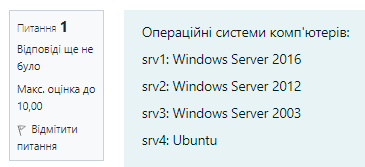
\includegraphics[width=5.93472in,height=3.59375in]{media/image2.emf}} \\
\multicolumn{3}{@{}>{\raggedright\arraybackslash}p{(\columnwidth - 4\tabcolsep) * \real{1.0000} + 4\tabcolsep}@{}}{%
\begin{minipage}[t]{\linewidth}\raggedright
\hypertarget{ux433ux440ux430ux444ux456ux43a-ux432ux456ux434ux43dux43eux441ux43dux43eux457-ux43fux43eux445ux438ux431ux43aux438-ux43eux431ux447ux438ux441ux43bux435ux43dux43dux44f}{%
\section{4.3. Графік відносної похибки
обчислення}\label{ux433ux440ux430ux444ux456ux43a-ux432ux456ux434ux43dux43eux441ux43dux43eux457-ux43fux43eux445ux438ux431ux43aux438-ux43eux431ux447ux438ux441ux43bux435ux43dux43dux44f}}

Вісь «Y»: колонка «δ» із п.4.1.

Вісь «X»: колонка «\emph{N}» із п.4.1.
\end{minipage}} \\
\multicolumn{3}{@{}>{\raggedright\arraybackslash}p{(\columnwidth - 4\tabcolsep) * \real{1.0000} + 4\tabcolsep}@{}}{%
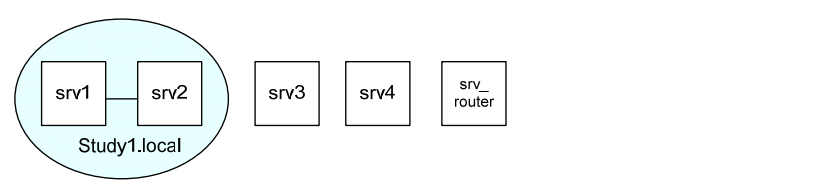
\includegraphics[width=5.95139in,height=3.82083in]{media/image3.emf}} \\
\multicolumn{3}{@{}>{\raggedright\arraybackslash}p{(\columnwidth - 4\tabcolsep) * \real{1.0000} + 4\tabcolsep}@{}}{%
\begin{minipage}[t]{\linewidth}\raggedright
\hypertarget{ux432ux438ux441ux43dux43eux432ux43eux43a}{%
\section{Висновок}\label{ux432ux438ux441ux43dux43eux432ux43eux43a}}

Висновок має давати відповіді на такі питання: Що зроблено? Як зроблено?
Що це дало?

Подати наближені значення або інтервали \emph{N}, в яких похибка прямує
до нуля.
\end{minipage}} \\
\multicolumn{3}{@{}>{\raggedright\arraybackslash}p{(\columnwidth - 4\tabcolsep) * \real{1.0000} + 4\tabcolsep}@{}}{%
У лабораторній роботі визначено суму послідовності чисел на основі їх
циклічного додавання та обчислено абсолютну і відносну похибки
одержаного результату. Програму написано мовою Python, обчислення
похибок та побудову графіків виконано у MS Excel. Для \emph{a} = 0,189
похибка прямує до нуля для інтервалів \emph{N} = (300; 400), (1600;
1700), (3300; 3400), (6300; 6400).} \\
\end{longtable}
